\section*{FISICA 1 - Fabrizio Cei \hfill 20|02|2024}
\subsubsection*{Caso 1: Urto totalmente anelastico $\Delta E \neq 0$}
\begin{figure}[H]
\raggedleft
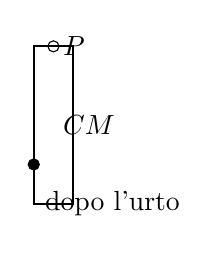
\begin{tikzpicture}
% sbarretta
\draw[thick] (2, -1) rectangle (2.5, 1);
\node at (2.7, 0) {$CM$};
% perno
\draw (2.25, 1) circle (2pt) node[right] {$P$};
% proiettile
\filldraw (2, -0.5) circle (2pt);
\node at (3, -1) {dopo l'urto};
\end{tikzpicture}
\end{figure}

$$ v' = \omega(b + L/2) = v_0 - \frac{2 M L^2 \omega}{3 m(L+2b)} $$
$$ \Rightarrow \omega = \frac{6 m v_0 (L+2b)}{4ML^2 + 3m(L+2b)^2} \quad \Rightarrow v' = \frac{v_0}{1 + \frac{4ML^2}{3m(L+2b)^2}} $$
$$ \Rightarrow \Delta E = - \frac{2 M m L^2 v_0^2}{4ML^2 + 3m(L+2b)^2} \quad \Rightarrow \Delta p = m v_0 \left[ \frac{6ML(b - L/6)}{4ML^2 + 3m(L+2b)^2} \right] $$

\subsubsection*{Caso 2: Urto totalmente elastico $\Delta E = 0$}
\begin{figure}[H]
\raggedleft
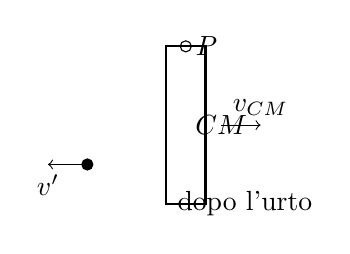
\begin{tikzpicture}
% sbarretta
\draw[thick] (2, -1) rectangle (2.5, 1);
\node at (2.7, 0) {$CM$};
\draw[->] (2.7, 0) -- (3.2, 0) node[above] {$v_{CM}$};
% perno
\draw (2.25, 1) circle (2pt) node[right] {$P$};
% proiettile
\filldraw (1, -0.5) circle (2pt);
\draw[->] (1, -0.5) -- (0.5, -0.5) node[below] {$v'$};
\node at (3, -1) {dopo l'urto};
\end{tikzpicture}
\end{figure}

$$ \frac{1}{2} + \frac{2ML^2}{3m(L+2b)^2} - \frac{2v_0}{\omega(L+2b)} = 0 \text{ affinché } \Delta E = 0 $$
$$ \Rightarrow \omega = \frac{12 m v_0 (L+2b)}{4ML^2 + 3m(L+2b)^2} $$
$$ \Rightarrow v' = v_0 \left( 1 - \frac{8 M L^2}{4ML^2 + 3m(L+2b)^2} \right) $$
$$ \Rightarrow \Delta p = m v_0 \left[ \frac{12 M L(b - L/6)}{4ML^2 + 3m(L+2b)^2} \right] $$

$\bar{b} = -b \hat{y}$ \\
$\Downarrow$ \\
$\bar{b} = L/2 \Rightarrow b = -L/2$

\subsubsection*{Caso 3: urto nel perno $\bar{b} = L/2$}
\paragraph*{3.1 (anelastico)}
$$ \Rightarrow \omega = 0 \quad \Rightarrow v' = 0 \quad \Rightarrow \Delta E = - \frac{1}{2} m v_0^2 \quad \Rightarrow \Delta p = - m v_0 $$

\paragraph*{3.2 (elastico)}
$$ \Rightarrow \omega = 0 \quad \Rightarrow v' = -v_0 \quad \Rightarrow \Delta p = -2 m v_0 $$

\subsection*{EQUILIBRIO DI UN CORPO RIGIDO}
Le forze applicate su un punto di applicazione hanno tutte l'origine comune quindi $\Sigma \bar{\tau}_i^{ext} = \Sigma_i \bar{r}_i \times \bar{F}_i^{ext} = \bar{r} \times \Sigma \bar{F}_i^{ext} = 0$ se $\Sigma_i \bar{F}_i^{ext} = 0$ (PUNTO MATERIALE) quindi è sufficiente che $\Sigma_i \bar{F}_i^{ext} = 0$. Invece nel CORPO RIGIDO essendo esteso e finito, le forze possono avere punti di applicazione diversi, quindi sono necessarie 2 condizioni:
$$ \begin{cases}
\Sigma \bar{F} = 0 \\
\Sigma \bar{\tau} = 0 \text{ (rispetto a un generico polo)}
\end{cases} \Rightarrow 6 \text{ equazioni per } 6 \text{ d.o.f.} $$

\subsubsection*{Caso 1: COPPIA DI FORZE}
esempio di verifica
$||\bar{F}_1|| = ||\bar{F}_2||$, $||\bar{r}_1|| = ||\bar{r}_2|| = L/2$

\begin{figure}[H]
\raggedleft
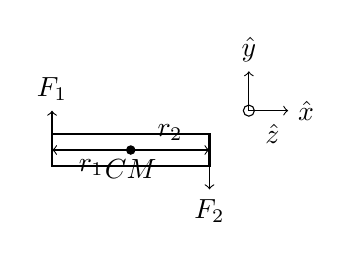
\begin{tikzpicture}
% sbarretta
\draw[thick] (2, -0.2) rectangle (4, 0.2);
\filldraw (3, 0) circle (1.5pt) node[below] {$CM$};
% forze
\draw[->] (2, -0.2) -- (2, 0.5) node[above] {$F_1$};
\draw[->] (4, 0.2) -- (4, -0.5) node[below] {$F_2$};
\draw[->] (3, 0) -- (2, 0) node[midway, below] {$r_1$};
\draw[->] (3, 0) -- (4, 0) node[midway, above] {$r_2$};
% assi
\draw[->] (4.5, 0.5) -- (5, 0.5) node[right] {$\hat{x}$};
\draw[->] (4.5, 0.5) -- (4.5, 1) node[above] {$\hat{y}$};
\draw[->] (4.5, 0.5) circle (2pt);
\node at (4.8, 0.2) {$\hat{z}$};
\end{tikzpicture}
\end{figure}

- $\Sigma \bar{F}_i = \bar{F}_1 + \bar{F}_2 = \bar{F}_1 + (-\bar{F}_1) = 0 \text{ \checkmark } \Rightarrow \bar{a}_{CM} = 0$
- $\Sigma_i \bar{\tau}_i = \bar{\tau}_1 + \bar{\tau}_2 = (\bar{r}_1 \times \bar{F}_1) + (\bar{r}_2 \times \bar{F}_2) = -\frac{L}{2} F_1 \hat{z} - \frac{L}{2} F_2 \hat{z} = -L F \hat{z} \neq 0 \text{ \xmark}$
$$ \bar{\alpha}_{CM} = \frac{\bar{\tau}_{CM}}{I_{CM}} = \frac{(-L F \hat{z})}{M L^2/12} = - \frac{12 F \hat{z}}{M L} \neq 0 $$
